\subsection{A Non-Variable Graph Implementation}
\begin{frame}[fragile]{\insertsubsection}
	\begin{tiny}
		\begin{columns}
			\column{.45\textwidth}
\begin{lstlisting}
public class Graph {
	List nodes = new ArrayList();
	List edges = new ArrayList();

	Edge add(Node n, Node m) {
		Edge e = new Edge(n, m);
		nodes.add(n); nodes.add(m); edges.add(e);
		e.weight = new Weight();
		return e;
	}
	Edge add(Node n, Node m, Weight w) {
		Edge e = new Edge(n, m);
		nodes.add(n); nodes.add(m); edges.add(e);
		e.weight = w;
		return e;
	}
	void print() {
		for (int i = 0; i < edges.size(); i++) {
			((Edge) edges.get(i)).print();
		}
	}
}
\end{lstlisting}
\begin{lstlisting}
public class Color {
	static void setDisplayColor(Color c) {...}
}
\end{lstlisting}	
			\column{.45\textwidth}
\begin{lstlisting}
public class Node {
	int id = 0;
	Color color = new Color();

	void print() {
		Color.setDisplayColor(color);
		System.out.print(id);
	}
}
\end{lstlisting}
\begin{lstlisting}
public class Edge {
	Node a, b;
	Weight weight = new Weight();

	Edge(Node _a, Node _b) {
		a = _a; b = _b;
	}
	void print() {
		a.print(); b.print();
		weight.print();
	}
}
\end{lstlisting}
\begin{lstlisting}
public class Weight {
	void print() {...}
}
\end{lstlisting}
		\end{columns}
	\end{tiny}
\end{frame}

\begin{frame}[fragile]{``Symbolic'' Feature Traces}
	\begin{tiny}
		\begin{columns}
			\column{.45\textwidth}
\begin{lstlisting}
public class Graph {
	List nodes = new ArrayList();
	List edges = new ArrayList();

	Edge add(Node n, Node m) {
		Edge e = new Edge(n, m);
		nodes.add(n); nodes.add(m); edges.add(e);
		@e.weight = new Weight();@
		return e;
	}
	@Edge add(Node n, Node m, Weight w) {
		Edge e = new Edge(n, m);
		nodes.add(n); nodes.add(m); edges.add(e);
		e.weight = w;
		return e;
	}@
	void print() {
		for (int i = 0; i < edges.size(); i++) {
			((Edge) edges.get(i)).print();
		}
	}
}
\end{lstlisting}
\begin{lstlisting}
~public class Color {
	static void setDisplayColor(Color c) {...}
}~
\end{lstlisting}	
			\column{.45\textwidth}
\begin{lstlisting}
public class Node {
	int id = 0;
	~Color color = new Color();~

	void print() {
		~Color.setDisplayColor(color);~
		System.out.print(id);
	}
}
\end{lstlisting}
\begin{lstlisting}
public class Edge {
	Node a, b;
	@Weight weight = new Weight();@

	Edge(Node _a, Node _b) {
		a = _a; b = _b;
	}
	void print() {
		a.print(); b.print();
		@weight.print();@
	}
}
\end{lstlisting}
\begin{lstlisting}
@public class Weight {
	void print() {...}
}@
\end{lstlisting}
		\end{columns}
	\end{tiny}
\end{frame}

\subsection{Adding Variability: A Basic Idea}
\begin{frame}[fragile]{\insertsubsection}
		\begin{columns}
			\column{.45\textwidth}
				\mynote{}{
					Conditional statements, controlled by configuration parameters (``feature toggles'').
				}
				\vspace{5mm}
\begin{tiny}
\begin{lstlisting}
public class Graph {
	...
	Edge add(Node n, Node m) {
		Edge e = new Edge(n, m);
		nodes.add(n); nodes.add(m); edges.add(e);
		@if (WEIGHTED) { e.weight = new Weight(); }@
		return e;
	}
	@Edge add(Node n, Node m, Weight w) {
		if (!WEIGHTED) { throw new RuntimeException(); }
		Edge e = new Edge(n, m);
		nodes.add(n); nodes.add(m); edges.add(e);
		e.weight = w;
		return e;
	}@
	...
}
\end{lstlisting}
\end{tiny}	
			\column{.45\textwidth}
\begin{tiny}
\begin{lstlisting}
public class Node {
	~Color color;~
	...
	Node(){
		~if (COLORED) { color = new Color(); }~
	}
	void print() {
		~if (COLORED) { Color.setDisplayColor(color); }~
		System.out.print(id);
	}
}
\end{lstlisting}
\begin{lstlisting}
public class Edge {
	@Weight weight;@ 
	...
	Edge(Node _a, Node _b) {
		a = _a; b = _b;
		@if (WEIGHTED) { weight = new Weight(); }@
	}
	void print() {
		a.print(); b.print();
		@if (WEIGHTED) { weight.print(); }@
	}
}
\end{lstlisting}
\end{tiny}	
		\end{columns}
\end{frame}

\subsection{Global Variables}
\begin{frame}[fragile]{\insertsubsection}
		\begin{columns}
			\column{.45\textwidth}
\begin{tiny}
\begin{lstlisting}
public class Config {
	~public static boolean COLORED = true;~
	@public static boolean WEIGHTED = false;@
}
\end{lstlisting}
\begin{lstlisting}
public class Graph {
	...
	Edge add(Node n, Node m) {
		Edge e = new Edge(n, m);
		nodes.add(n); nodes.add(m); edges.add(e);
		@if (Config.WEIGHTED) { e.weight = new Weight(); }@
		return e;
	}
	@Edge add(Node n, Node m, Weight w) {
		if (!Config.WEIGHTED) { throw new RuntimeException(); }
		Edge e = new Edge(n, m);
		nodes.add(n); nodes.add(m); edges.add(e);
		e.weight = w;
		return e;
	}@
	...
}
\end{lstlisting}
\end{tiny}	
			\column{.45\textwidth}
\begin{tiny}
\begin{lstlisting}
public class Node {
	~Color color;~
	...
	Node(){
		~if (Config.COLORED) { color = new Color(); }~
	}
	void print() {
		~if (Config.COLORED) { Color.setDisplayColor(color); }~
		System.out.print(id);
	}
}
\end{lstlisting}
\begin{lstlisting}
public class Edge {
	@Weight weight;@
	...
	Edge(Node _a, Node _b) {
		a = _a; b = _b;
		@if (Config.WEIGHTED) { weight = new Weight(); }@
	}
	void print() {
		a.print(); b.print();
		@if (Config.WEIGHTED) { weight.print(); }@
	}
}
\end{lstlisting}
\end{tiny}	
		\end{columns}
\end{frame}

\begin{frame}[fragile]{Special Case: Immutable Global Variables}
		\begin{columns}
			\column{.45\textwidth}
\begin{tiny}
\begin{lstlisting}
public class Config {
	~public static final boolean COLORED = true;~
	@public static final boolean WEIGHTED = false;@
}
\end{lstlisting}
\begin{lstlisting}
public class Graph {
	...
	Edge add(Node n, Node m) {
		Edge e = new Edge(n, m);
		nodes.add(n); nodes.add(m); edges.add(e);
		@if (Config.WEIGHTED) { e.weight = new Weight(); }@
		return e;
	}
	@Edge add(Node n, Node m, Weight w) {
		if (!Config.WEIGHTED) { throw new RuntimeException(); }
		Edge e = new Edge(n, m);
		nodes.add(n); nodes.add(m); edges.add(e);
		e.weight = w;
		return e;
	}@
	...
}
\end{lstlisting}
\end{tiny}	
			\column{.45\textwidth}
				\mynote{}{ 
					\begin{itemize}
						\item {\bf Idea:} Static configuration when configuration parameters are known at compile time.
					\end{itemize}					
					\begin{itemize}
						\item {\bf Advantage:} Compiler optimizations may remove dead code.
					\end{itemize}					
					\begin{itemize}
						\item {\bf Disadvantage:} No external configuration by the end-user.
					\end{itemize}
				}
		\end{columns}
\end{frame}

\subsection{Method Parameters and Parameter Passing}
\begin{frame}[fragile]{\insertsubsection}
		\begin{columns}
			\column{.45\textwidth}
\begin{tiny}
\begin{lstlisting}
public class Graph {
	@boolean weighted;@
	~boolean colored;~
	...
	Graph(@boolean _weighted@, ~boolean _colored~) {
		@weighted = _weighted;@
		~colored = _colored;~
	}
	
	Edge add(Node n, Node m) {
		Edge e = new Edge(n, m, @weighted@);
		nodes.add(n); nodes.add(m); edges.add(e);
		@if (weighted) { e.weight = new Weight(); }@
		return e;
	}
	...
}
\end{lstlisting}
\begin{lstlisting}
public class Edge {
	@boolean weighted;@
	@Weight weight;@ 
	...
	Edge(Node _a, Node _b, @boolean weighted@) {
		a = _a; b = _b;
		@if (weighted) { weight = new Weight(); }@
	}
	...
}
\end{lstlisting}
\end{tiny}	
			\column{.45\textwidth}
				\mynote{Idea}{ 
					\begin{itemize}
						\item A class exposes its configuration parameters as part of its interface (i.e., method parameters).
						\item Parameter values are passed along method invocations.
					\end{itemize}
				}				
				\mynote{Discussion}{ 
					\begin{itemize}
						\item {\bf Advantage:} Different instantiations (e.g., colored and uncolored graphs) within in the same program.
					\end{itemize}					
					\begin{itemize}
						\item {\bf Disadvantage:} May lead to methods with many parameters (code smell!).
					\end{itemize}
				}
		\end{columns}
\end{frame}

\subsection{Reconfiguration at Runtime?}
\begin{frame}[fragile]{\insertsubsection}
		\begin{columns}
			\column{.45\textwidth}
\begin{tiny}
\begin{lstlisting}
public class Config {
	~public static boolean COLORED = false;~
	@public static boolean WEIGHTED = false;@
}

\end{lstlisting}
\begin{lstlisting}
public class Node {
	~Color color;~
	...
	Node(){
		~if (Conf.COLORED) { 
			color = new Color(); 
		}~
	}
	void print() {
		~if (Conf.COLORED) { 
			Color.setDisplayColor(color); 
		}~
		System.out.print(id);
	}
}
\end{lstlisting}
\end{tiny}	
			\column{.45\textwidth}
				\mynote{Idea}{ 
					\begin{itemize}
						\item Alter feature selection without stopping and restarting the program.
					\end{itemize}
				}				
				\mynote{Discussion}{ 
					\begin{itemize}
						\item Feature-specific code may depend on certain initialization steps or assume certain invariants.
						\item Just updating the values of configuration parameters does not update the current state of the program.
					\end{itemize}
				}
		\end{columns}
\end{frame}

\subsection{Code Scattering}
\begin{frame}{Problem: Code Scattering}
	\begin{center}
		\vspace[-2mm}
		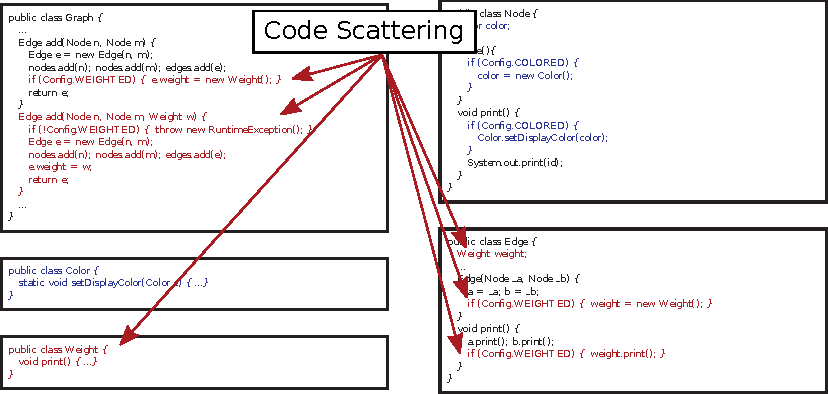
\includegraphics[scale=1.0]{scattering}
	\end{center}
\end{frame}

\subsection{Code Tangling}
\begin{frame}{Problem: Code Tangling}
	\begin{center}
		\vspace[-2mm}
		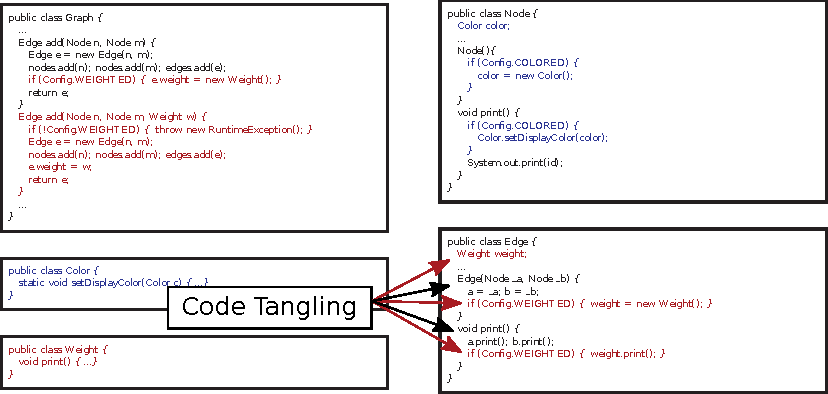
\includegraphics[scale=1.0]{tangling}
	\end{center}
\end{frame}

\subsection{Code Replication}
\begin{frame}{Problem: Code Replication}
	\begin{center}
		\vspace[-2mm}
		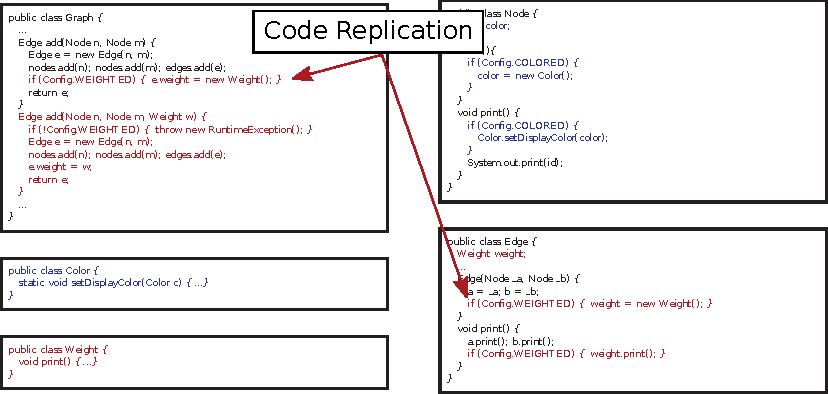
\includegraphics[scale=1.0]{replication}
	\end{center}
\end{frame}